% Created:  Fri 27 Jun 2014 11:24 AM
% Modified: Wed 23 Jul 2014 05:08 PM
% @author Josh Wainwright
% File name : quadtree.tex

\section{Quadtrees}
\label{sec:quadtrees}

Since the simple grid method described in section~\ref{sec:simple_grid_method}
performs slowly and does not offer good cluster analysis, a different approach
is needed. The chosen method is to use a quadtree data structure.

Quadtrees are a type of recursive abstract data type in the form of a tree
where every node has exactly zero or four children. A node with zero children
is a leaf and contains some information, value or quantity. A node with four
children is not a leaf and cannot hold information.

Quadtrees are often used in image processing since the four children of the
root node can naturally represent the four quadrants of the image; upper left,
upper right, lower left and lower right. Since each of these children is also a
quadtree, the image can be subdivided to any arbitrary depth. From this point,
information about the image can be ``seen'' more easily by the computer and
statistics calculated.

\subsection{Quadtree Definitions}
\label{sub:quadtree_definitions}

It is useful to define a few terms that shall be used in the context of
quadtrees. Many of these are identical to the definitions more commonly applied
to binary trees.

\begin{description}
	\item[Node] (Cell) A leaf in the tree which holds a number of points.
	\item[Root] The node at the topmost position in the tree.
	\item[Child] One of the four nodes that are beneath a given node for which
		there is a direct path of length 1 between this node and it.
	\item[Height] The length of the longest path from the root node to one of
		the leaf nodes.
	\item[Depth] The length of the path from a given node up to the root.
	\item[Completeness] A quadtree is `complete' when each of the root node's
		four children have the same height. In this case, the number of leaves
		in the tree is a maximum.
	\item[Quadtree Code] (Code) The unique binary number assiged to a node by
		adding its position with respect to its siblings to the code of its
		parent.
\end{description}

\subsection{Code Orderings}
\label{sub:code_orderings}

In order to identify a node uniquely in the tree, each node is given a code
that is built up from it's parent code plus some value that identifies it
among it's siblings. The root node is usually chosen to have an empty code so
that the first four children are given the first level codes.

The choice of what order to label the children is important if the order
in which the nodes are placed is important. For spatial indexing, for example,
each node represents a quadrant in two dimensional space, so being able to
traverse the children in a sensible and predictable way is essential.

\subsubsection[Morton Order]{Morton Order (Z-Order)}
\label{ssub:morton_code_z_order_}

Perhaps the most natural order to give to the values in a spatial quadtree is
to number them from 1 to 4, left to right, top to bottom. This can be made
more appropriate for a computer to use by numbering from 0 to 3. This is
called Morton Order\cite{mortoncomputer} or Z-order because of the resulting
path that would be followed by traversing the nodes in order,
Figure~\ref{fig:traverse-z-order.pdf}. This has several useful features.

\begin{enumerate}
	\item First, the numbers can be converted to base 2:
	\begin{itemize}
		\item 0 becomes 00
		\item 1 becomes 01
		\item 2 becomes 10 and
		\item 3 becomes 11.
	\end{itemize}

	\item This has advantages since binary is very efficient for computers to
	work with and allows certain tricks to be employed (see Morton order
	coordinates).

	\item Also, this numbering system is easily extendible to any depth of
	tree that can be imagined.

	\begin{enumerate}
		\item The root, as mentioned before, is given no value,
		\item each of the children are numbered {00} through 11.

		\item the children of these children are numbered 00 to 11 with the
		parent as a prefix. So the children of node 00 are 0000, 0001, 0010
		and 0011. Likewise, the children of 11 are 1100, 1101, 1110 and 1111.

		\item The children are always numbered in the same order. If starting
		at the top and going top to bottom and left to right, this is
		maintained for all children.
	\end{enumerate}
\end{enumerate}

This method of numbering is simple and so acceptable for the standard uses of
quadtrees, but it was found to be difficult to work with in a spatial context
when information about neighbouring cells is needed. The steps required to
calculate the neighbours of any given cell are reasonably complex and so would
add computational and time complexity to calculations performed on the tree.

\subsubsection*{Morton Order Coordinates}
\label{ssub:Morton Order Coordinates}

Another useful feature of the Morton ordering is the simple conversion from
quadtree code to Cartesian coordinate notation. The steps to convert to
coordinate form are:

\begin{enumerate}
	\item Ensure the code is in binary format with two bits for each level of
		the tree,
	\item \emph{de-interleave} the bits of the code (starting with the first
		being given to the $y$-axis, assign bits to the $y$ and $x$ axes
		building up a binary value for each),
	\item convert the resulting two binary value to decimal to give a standard
		decimal $(x,y)$ coordinate.
\end{enumerate}

This method means that it is very easy to calculate an arbitrary number of
nodes in any direction by simply converting the code for a node to coordinates,
adding or subtracting the number of positions to move in the $x$ and $y$
directions and then converting back to quadtree code representation by
following the algorithm above in the reverse order.

Of course, this method has no knowledge of the structure of the quadtree being
used and so only provides the code of the node that would occupy the space at
the given coordinate. That node might not exist---the tree might not extend
deep enough, so the node in that position is larger than expected; or the tree
might be deeper at that location meaning the node is smaller. In these cases,
there are a number of options as to how to find the correct node for the code:

\begin{itemize}
	\item The code can be shortened and/or lengthened and the resulting adapted
		code checked to see if it is in the tree. This trial and error method
		can be fastest when there is a limit on the depth range allowed when
		%TODO find correct reference
		searching (see Section~\ref{sec:}).
	\item The tree can be traversed to find the nearest node to the expected
		code reference.
\end{itemize}

\subsubsection{Hilbert Order}
\label{ssub:hilbert_order}

One of the reasons the Z-order above becomes difficult to work with is that
the resulting path from traversing the nodes in-order has to make large jumps
and so cells which are numbered next to each other may, in fact, not be near
each other in the image.

A number of routes exist that avoid this jumping around the image. These are
based on space filling curves which have the property of being a simple
recursive pattern that visits every point in a 2D space exactly once. These
curves were first discovered in the early 1900's and described mathematically
by D. Hilbert\cite{hilbert1970stetige}. One of the curves that Hilbert found,
the Hilbert Curve, is particularly useful since it can be represented in the
simplest level in a two by two square which is then recursively repeated for
each quadrant of that first square---exactly as the quadtree does.

The path that the traversal of points follows becomes fairly complicated,
Figure~\ref{fig:traverse-hilbert-order.pdf}. This means, again, that the
calculation of neighbours becomes difficult.

\begin{figure}[tbhp]
    \centering
    \begin{subfigure}[b]{0.42\linewidth}
        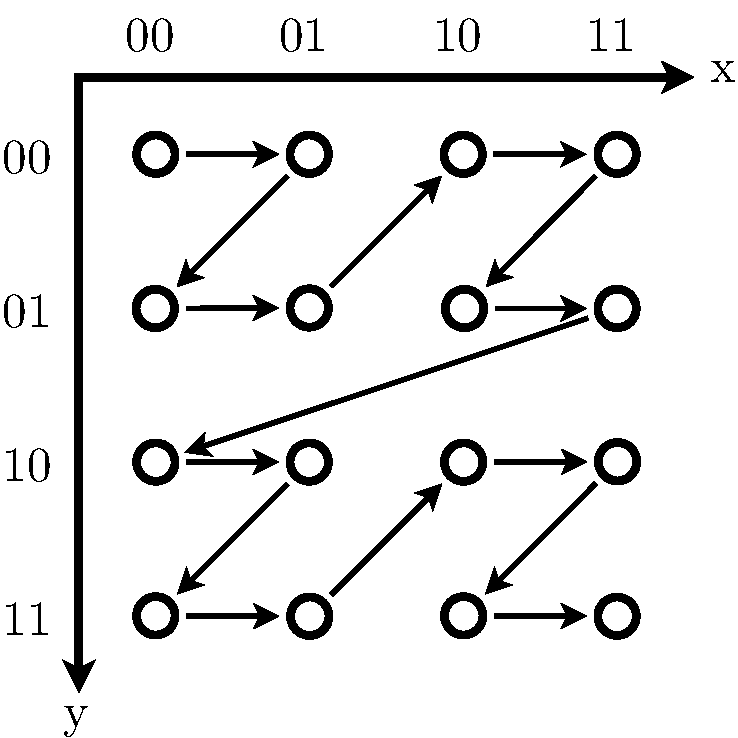
\includegraphics[width=\textwidth]{traverse-z-order.pdf}
        \caption{} \label{fig:traverse-z-order.pdf}
    \end{subfigure}%
    \quad
    \begin{subfigure}[b]{0.42\linewidth}
        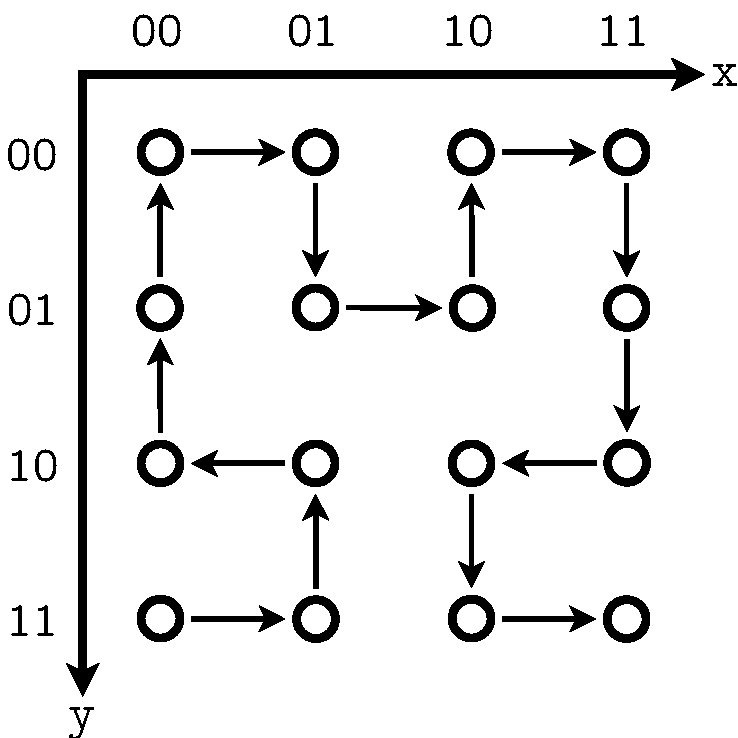
\includegraphics[width=\textwidth]{traverse-hilbert-order.pdf}
        \caption{} \label{fig:traverse-hilbert-order.pdf}
    \end{subfigure}
    \\[0.2cm]
    \begin{subfigure}[b]{0.42\linewidth}
        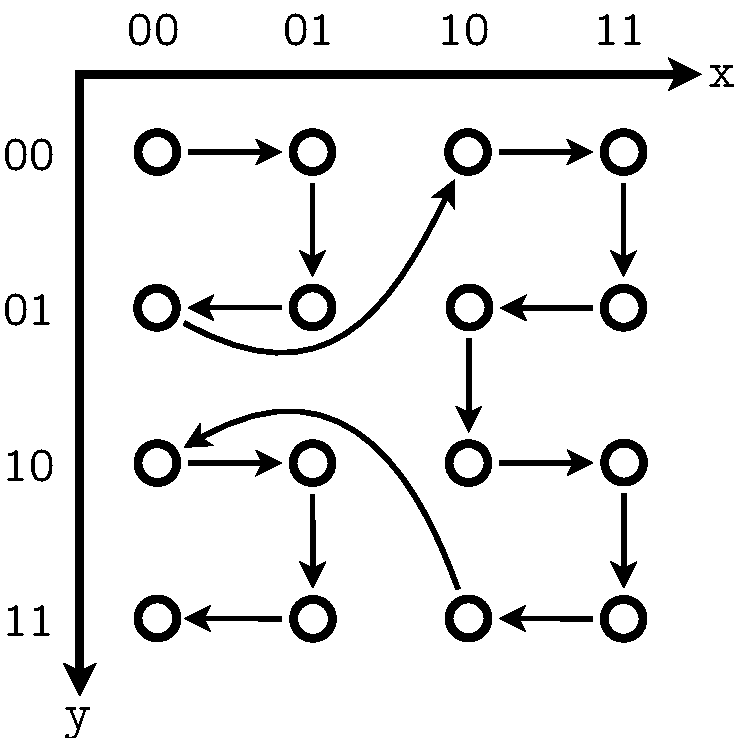
\includegraphics[width=\textwidth]{traverse-gray-order.pdf}
        \caption{} \label{fig:traverse-gray-order.pdf}
    \end{subfigure}%
    \quad
    \begin{subfigure}[b]{0.42\linewidth}
        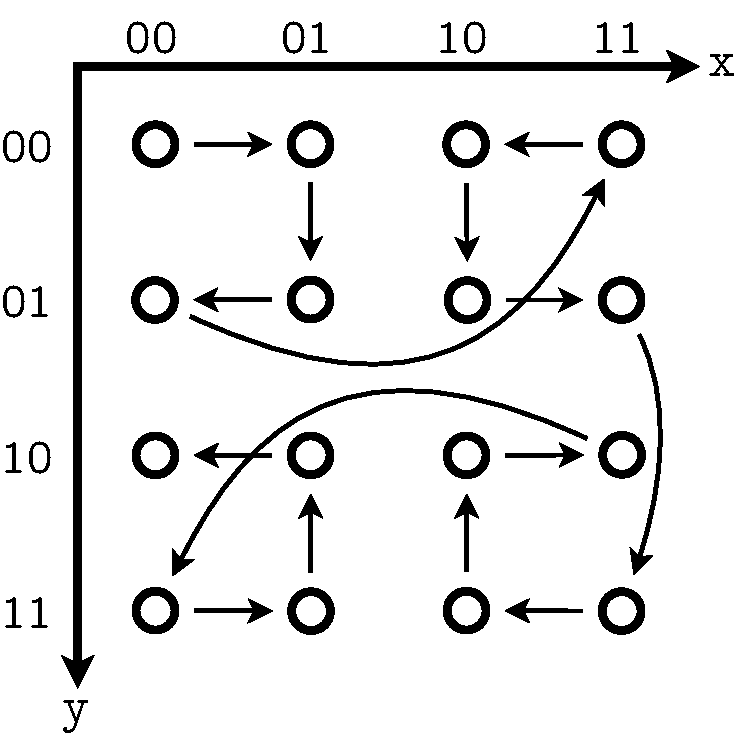
\includegraphics[width=\textwidth]{traverse-modgray-order.pdf}
        \caption{}\label{fig:traverse-modgray-order.pdf}
    \end{subfigure}
    \caption{A selection of possible tree traversal orderings. Each of theses
    is, more formally, a space filling curve which is a direct, unique mapping
    from a 2D grid to a 1D array. \subref{fig:traverse-z-order.pdf} shows
    Z-order, \subref{fig:traverse-hilbert-order.pdf} shows Hilbert order,
    \subref{fig:traverse-gray-order.pdf} shows Gray code order and
    \subref{fig:traverse-modgray-order.pdf} shows the modified Gray code order
    developed for this project.} \label{fig:order_traversals}
\end{figure}

\subsubsection{Gray Codes}
\label{ssub:gray_codes}

The Gray Code\cite{gray1953pulse}, developed by Frank Gray in 1953, was
originally designed to reduce the error rate produced by mechanical
electronics. The code is a variation on binary where each step when counting
up changes only a single bit at a time. This meant that electromechanical
apparatus was less likely to make a mistake or generate errors since the
actions required to count from one to two required only a single bit change,
rather than two, as would be required for binary counting. When using just two
bits, i.e., counting from zero to three, the steps are very similar to binary,
(00, 01, 11, 10).

The path that this follows is shown in
Figure~\ref{fig:traverse-gray-order.pdf}. This does not seem to provide any
benefits since there is now more jumping around the image space than with
Z-order and the neighbours are just as difficult to calculate as for Hilbert
Order. However, by using a different arrangement of the sub-trees, as the
Hilbert curve does, the leaf nodes group themselves in a very ordered
fashion. When arranged as in Figure~\ref{fig:traverse-modgray-order.pdf}
and~\ref{fig:modgray-traversal}, each cell is arranged such that

\begin{figure}[tbhp]
    \centering
    \begin{subfigure}[c]{0.41\linewidth}
        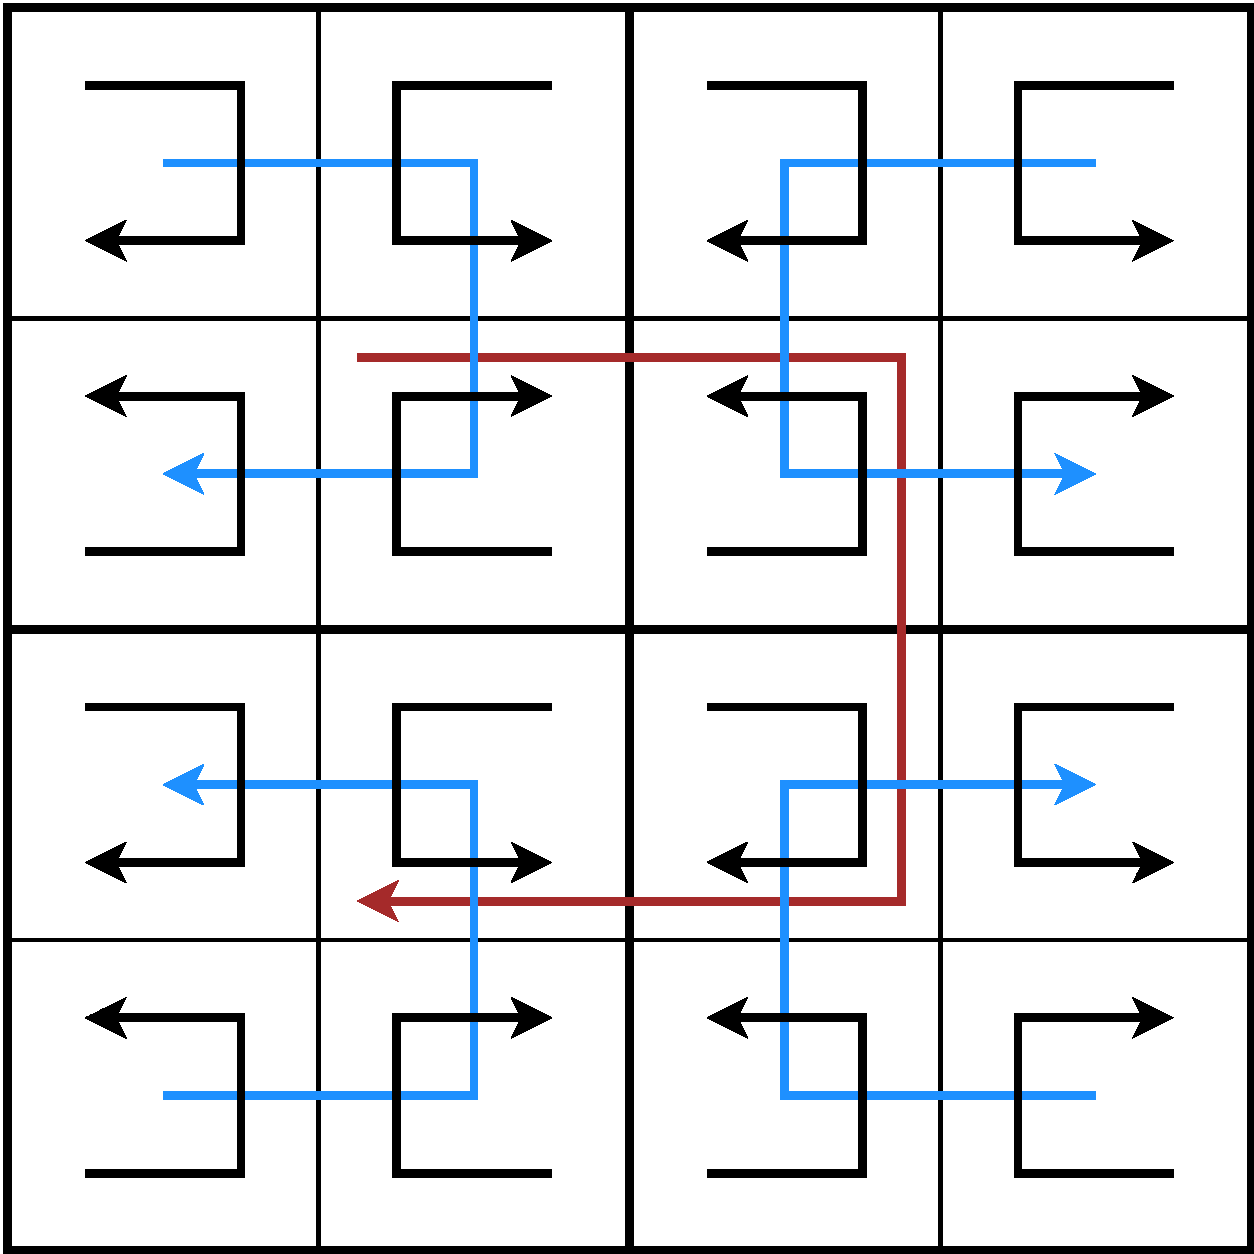
\includegraphics[width=\textwidth]{modgray-2-levels-arrows.pdf}
        \caption{}\label{fig:modgray-2-levels-arrows.pdf}
    \end{subfigure}%
    \quad
    \begin{subfigure}[c]{0.55\linewidth}
        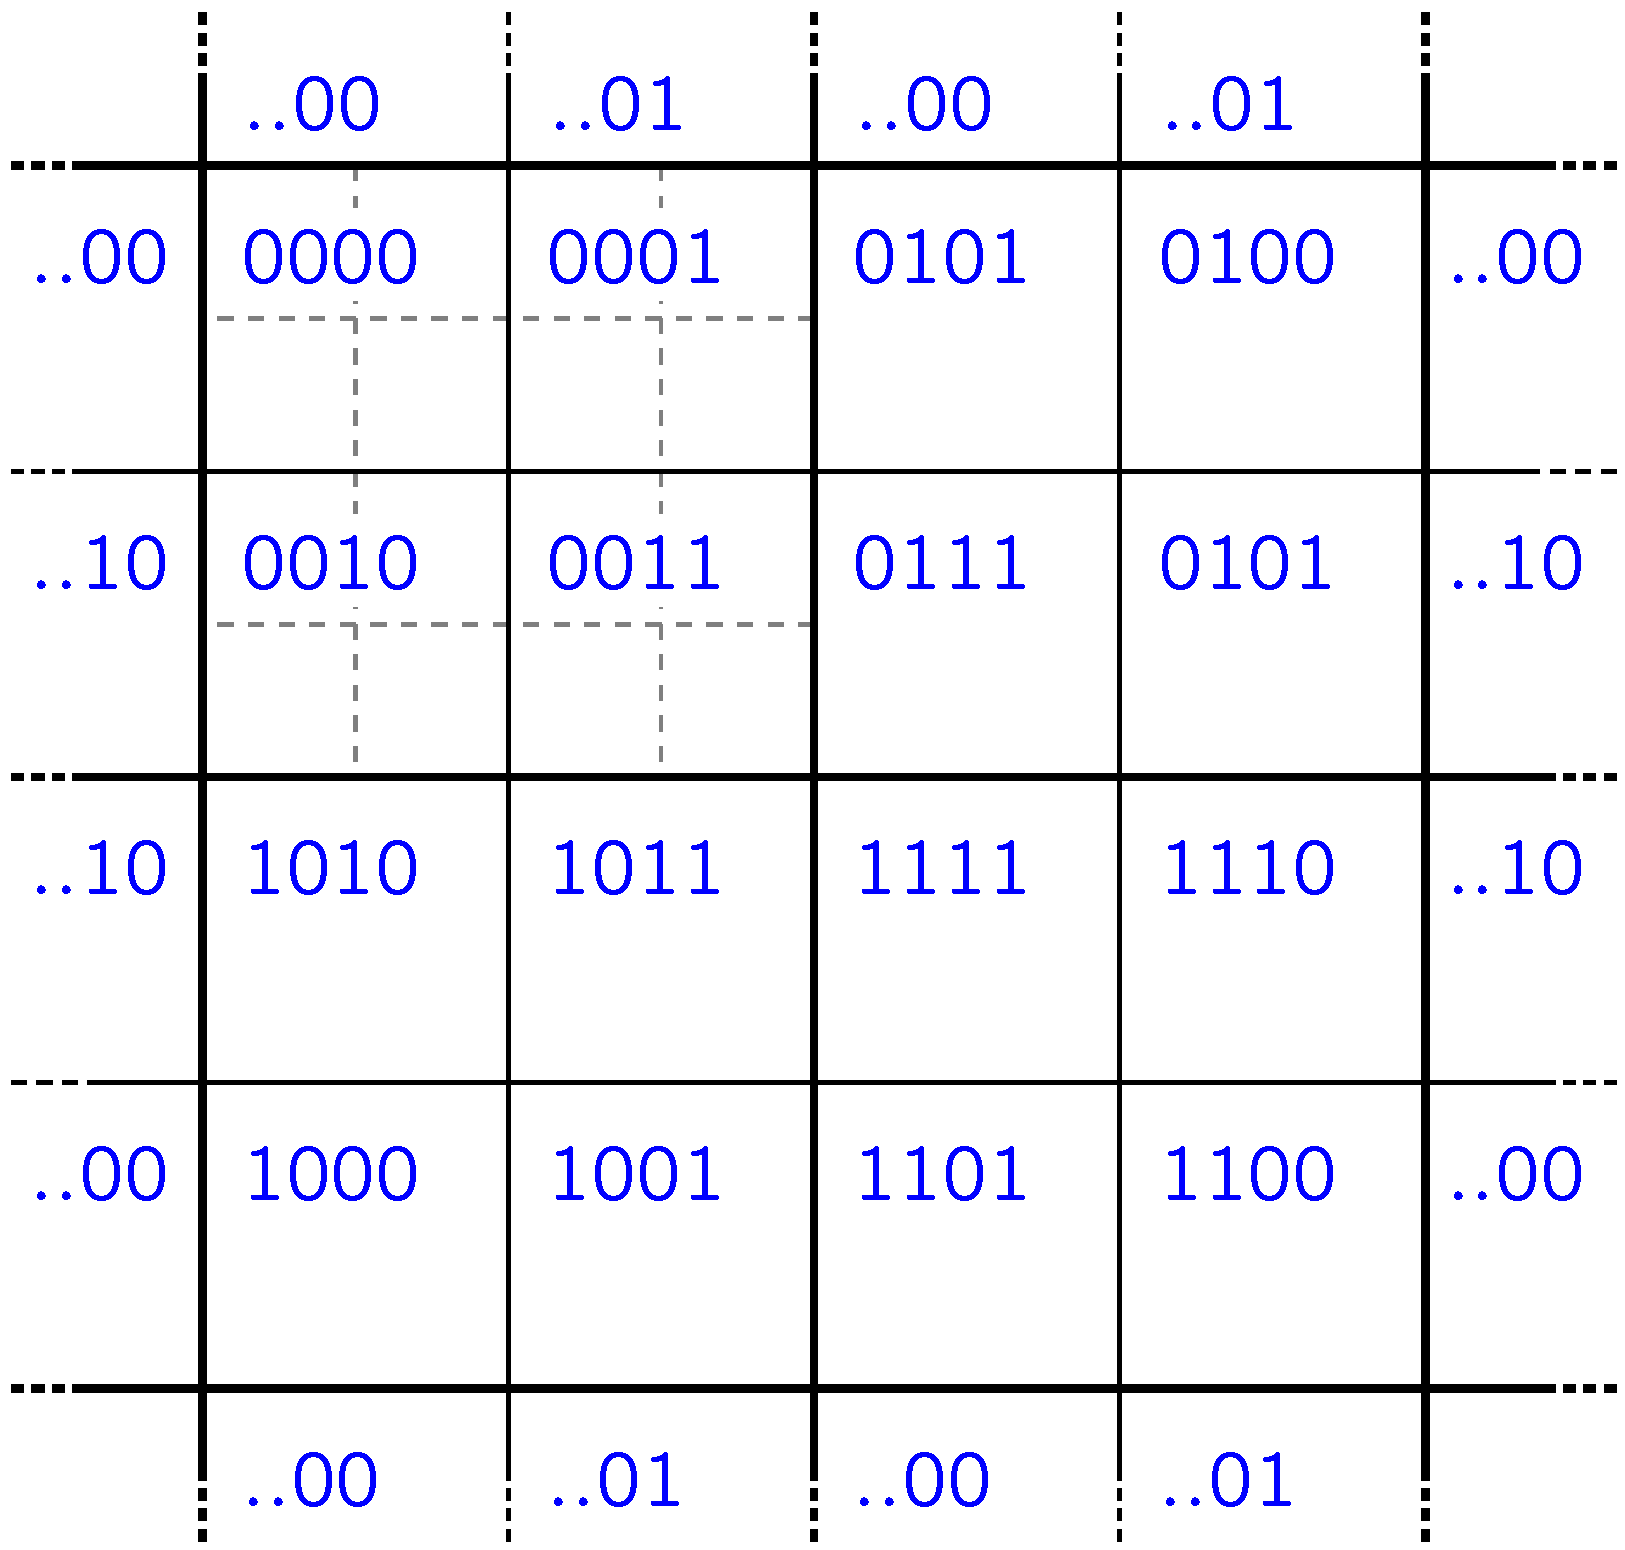
\includegraphics[width=\textwidth]{modgray-2-levels-numbers.pdf}
        \caption{}\label{fig:modgray-2-levels-numbers.pdf}
    \end{subfigure}
    \caption{The tree traversal that was developed for this project is a
    	variation of the Gray code order discussed in
    	Section~\ref{ssub:gray_codes}.  Instead of all sub-quadrants having the
    	same orientation, each is reflected in either the x- or y-axis,
    	\subref{fig:modgray-2-levels-arrows.pdf}. This has the advantage that
		neighbouring nodes have codes which differ by exactly one bit,
		\subref{fig:modgray-2-levels-numbers.pdf}.} \label{fig:modgray-traversal}
\end{figure}

\begin{figure}[tbhp]
	\centering
	\includegraphics[width=\linewidth]{modgray-steps.pdf}
	\caption{modgray-Steps}
	\label{fig:modgray-steps}
\end{figure}

Since the quadtree is a recursive data structure, it is necessary to be able
to maintain the correct orientation of child trees with respect to their
parents at the construction stage. It turns out that this is easy to achieve
and thus adapting it for each of the arrangements discussed above is simply a
matter of adjusting the next part of the code that is added for each of the
four children when creating them. Pseudo code to achieve this for the Morton
order and the modified Gray code order is shown in Listing
~\ref{code:child_construction}.

\begin{lstlisting}[caption={Code to generate children of the current quadtree
while maintaining the correct ordering.},label=code:child_construction]
// Constructor
Quadtree(max_x, max_y, code)

// Child creation,  Z-Order
t_l = new Quadtree(100, 100, this.code + "00");
t_r = new Quadtree(100, 100, this.code + "01");
b_l = new Quadtree(100, 100, this.code + "11");
b_r = new Quadtree(100, 100, this.code + "10");

// Child creation,  Gray Code
t_l = new Quadtree(100, 100, this.code + "00");
t_r = new Quadtree(100, 100, this.code + "01");
b_l = new Quadtree(100, 100, this.code + "10");
b_r = new Quadtree(100, 100, this.code + "11");

// Child creation, Modified Gray Code
if (pos == "tl") ) {
	new_code[0] = code + "00";
	new_code[1] = code + "01";
	new_code[2] = code + "10";
	new_code[3] = code + "11";

} else if (pos == "tr")) {
	new_code[0] = code + "01";
	new_code[1] = code + "00";
	new_code[2] = code + "11";
	new_code[3] = code + "10";

} else if (pos == "bl")) {
	new_code[0] = code + "10";
	new_code[1] = code + "11";
	new_code[2] = code + "00";
	new_code[3] = code + "01";

} else if (pos == "br")){
	new_code[0] = code + "11";
	new_code[1] = code + "10";
	new_code[2] = code + "01";
	new_code[3] = code + "00";
}
t_l = new Quadtree(100, 100, this.code + new_code[0]);
t_r = new Quadtree(100, 100, this.code + new_code[1]);
b_l = new Quadtree(100, 100, this.code + new_code[2]);
b_r = new Quadtree(100, 100, this.code + new_code[3]);
\end{lstlisting}

\subsection{Hash Table Implementation}
\label{sub:hash_table_implementation}

In order to speed up the subsequent operations applied to the quadtree
structure, it can be converted to a simpler, one dimensional data structure.
The method discussed above, to number the cells in a logical fashion based on
the code of the parent, can be viewed as a way to map the two dimensional image
to a single unique binary code, and hence to a one dimensional format. Thus,
the quadtree can be easily converted to an array structure by simply using the
key code as the array index.

As mentioned in Part~\ref{prt:data_structures}, this has the potential to
have a very poor space usage if the image is not densely populated (in which
case it is likely that few clusters would be identifiable anyway). Instead, an
implementation is created that makes use of the \emph{Hash Table} data
structure\cite{cormen2001introduction}. This allows the data structure to
increase in size dynamically as more space is needed, but also provides linear
time complexity for access and modification. The quadtree code is used as the
key for the hash table, and the data stored within the cell with that code is
the value.

Using this data structure means that several operations are significantly sped
up. For example, for the raw quadtree format, the steps required to check if a
given code is present involve traversing every node in the tree, thus linear
$O(n)$.  However, for a hash table, the hash function is used to get a hash of
the code to be checked and the appropriate location checked. If the codes
match, then the code does appear in the tree, a total of two operations,
constant $O(1)$.

Also, since the structure is defined recursively, it is not possible to
directly access a given location of the data. Instead it must be arrived at by
starting at the root, and, for every level, deciding which of the children the
destination exists in. This would be a time consuming step for a number of
operations, but the biggest effect would be when checking the neighbours of
cells since for every neighbour of every node, the tree must be traversed. This
is not an issue for the hash table since the single dimensional nature means
that data can be accessed directly anywhere.

Little spatial information should be lost during the conversion from quadtree
to hash table since this is all contained in the quadtree code assigned to the
node during the quadtree generation step.
